\documentclass{article}[18pt]
\ProvidesPackage{format}
%Page setup
\usepackage[utf8]{inputenc}
\usepackage[margin=0.7in]{geometry}
\usepackage{parselines} 
\usepackage[english]{babel}
\usepackage{fancyhdr}
\usepackage{titlesec}
\hyphenpenalty=10000

\pagestyle{fancy}
\fancyhf{}
\rhead{Sam Robbins}
\rfoot{Page \thepage}

%Characters
\usepackage{amsmath}
\usepackage{amssymb}
\usepackage{gensymb}
\newcommand{\R}{\mathbb{R}}

%Diagrams
\usepackage{pgfplots}
\usepackage{graphicx}
\usepackage{tabularx}
\usepackage{relsize}
\pgfplotsset{width=10cm,compat=1.9}
\usepackage{float}

%Length Setting
\titlespacing\section{0pt}{14pt plus 4pt minus 2pt}{0pt plus 2pt minus 2pt}
\newlength\tindent
\setlength{\tindent}{\parindent}
\setlength{\parindent}{0pt}
\renewcommand{\indent}{\hspace*{\tindent}}

%Programming Font
\usepackage{courier}
\usepackage{listings}
\usepackage{pxfonts}

%Lists
\usepackage{enumerate}
\usepackage{enumitem}

% Networks Macro
\usepackage{tikz}


% Commands for files converted using pandoc
\providecommand{\tightlist}{%
	\setlength{\itemsep}{0pt}\setlength{\parskip}{0pt}}
\usepackage{hyperref}

% Get nice commands for floor and ceil
\usepackage{mathtools}
\DeclarePairedDelimiter{\ceil}{\lceil}{\rceil}
\DeclarePairedDelimiter{\floor}{\lfloor}{\rfloor}

% Allow itemize to go up to 20 levels deep (just change the number if you need more you madman)
\usepackage{enumitem}
\setlistdepth{20}
\renewlist{itemize}{itemize}{20}

% initially, use dots for all levels
\setlist[itemize]{label=$\cdot$}

% customize the first 3 levels
\setlist[itemize,1]{label=\textbullet}
\setlist[itemize,2]{label=--}
\setlist[itemize,3]{label=*}

% Definition and Important Stuff
% Important stuff
\usepackage[framemethod=TikZ]{mdframed}

\newcounter{theo}[section]\setcounter{theo}{0}
\renewcommand{\thetheo}{\arabic{section}.\arabic{theo}}
\newenvironment{important}[1][]{%
	\refstepcounter{theo}%
	\ifstrempty{#1}%
	{\mdfsetup{%
			frametitle={%
				\tikz[baseline=(current bounding box.east),outer sep=0pt]
				\node[anchor=east,rectangle,fill=red!50]
				{\strut Important};}}
	}%
	{\mdfsetup{%
			frametitle={%
				\tikz[baseline=(current bounding box.east),outer sep=0pt]
				\node[anchor=east,rectangle,fill=red!50]
				{\strut Important:~#1};}}%
	}%
	\mdfsetup{innertopmargin=10pt,linecolor=red!50,%
		linewidth=2pt,topline=true,%
		frametitleaboveskip=\dimexpr-\ht\strutbox\relax
	}
	\begin{mdframed}[]\relax%
		\centering
		}{\end{mdframed}}



\newcounter{lem}[section]\setcounter{lem}{0}
\renewcommand{\thelem}{\arabic{section}.\arabic{lem}}
\newenvironment{defin}[1][]{%
	\refstepcounter{lem}%
	\ifstrempty{#1}%
	{\mdfsetup{%
			frametitle={%
				\tikz[baseline=(current bounding box.east),outer sep=0pt]
				\node[anchor=east,rectangle,fill=blue!20]
				{\strut Definition};}}
	}%
	{\mdfsetup{%
			frametitle={%
				\tikz[baseline=(current bounding box.east),outer sep=0pt]
				\node[anchor=east,rectangle,fill=blue!20]
				{\strut Definition:~#1};}}%
	}%
	\mdfsetup{innertopmargin=10pt,linecolor=blue!20,%
		linewidth=2pt,topline=true,%
		frametitleaboveskip=\dimexpr-\ht\strutbox\relax
	}
	\begin{mdframed}[]\relax%
		\centering
		}{\end{mdframed}}
\lhead{CT - Graphs}
\lstset{language=Python,
	basicstyle=\ttfamily,
	keywordstyle=\bfseries,
	showstringspaces=false,
	morekeywords={if, else, then, print, end, for, do, while},
	tabsize=4,
	mathescape=true
}

\begin{document}
\begin{center}
\underline{\huge Graph Traversing I}
\end{center}
\section{Graph Representations}
\begin{itemize}
	\item Humans understand graphs pictorially as a collection of vertices and edges
	\item For a computer to understand graphs it needs to be stored in a structured way
\end{itemize}
Two standard data structures to represent graphs:
\begin{itemize}
	\item A collection of adjacency lists
	\begin{itemize}
		\item For every vertex, a lined list with all its neighbours
		\item These lists are called adjacency lists
	\end{itemize}
	\item An adjacency matrix
	\begin{itemize}
		\item The vertices are (arbitrarily) numbered 1,2,3,...,n
		\item a square $n\times n$ matrix such that the element (i,j) is:
		\begin{itemize}
			\item equal to 1 if vertices i and j are adjacent
			\item equal to 0 otherwise
		\end{itemize}
	\end{itemize}
\end{itemize}
For undirected graphs:
\begin{itemize}
	\item The adjacency matrix is symmetric (the elements (i,j) and (j,i) are equal)
\end{itemize}
\section{Graph traversing}
\begin{itemize}
	\item Both data structures
	\begin{itemize}
		\item store only "local" information about the graph (i.e. adjacencies)
		\item The "global" information is provided implicitly
	\end{itemize}
	\item How can you know if the graph is \textbf{connected}?
	\begin{itemize}
		\item If you start at a specific vertex, can you reach every other vertex?
		\item If not, can you list the "reachable vertices"
	\end{itemize}
\end{itemize}
Where is the difficulty? -  we want to visit all accessible vertices but avoid running into "cycles"\\
\\
Algorithm to traverse a labyrinth:
\begin{itemize}
	\item Whenever you find an unvisited vertex continue to explore it from deeper
	\item If no more options, use a \textit{ball of string} to return to junctions that you previously saw but did not investigate
\end{itemize}
\section{Depth First Search (DFS)}
The depth first search algorithm:
\begin{lstlisting}
DFS(G,u)
visited[u]=1
print u
for each vertex $v\in$ Adj[u]
	if visited[v]==0 then
		DFS(G,v)
\end{lstlisting}
\begin{itemize}
	\item Initially all vertices are marked as "unvisited" i.e. visited[u]=0 for all vertices u
	\item When we visit a new vertex u
	\begin{itemize}
		\item We mark it as visited (line 1)
		\item We call (recursively) the same algorithm (DFS) for all unvisited neighbours v of u (lines 3-5)
	\end{itemize}
\end{itemize}
\section{DFS in action}
\begin{center}
	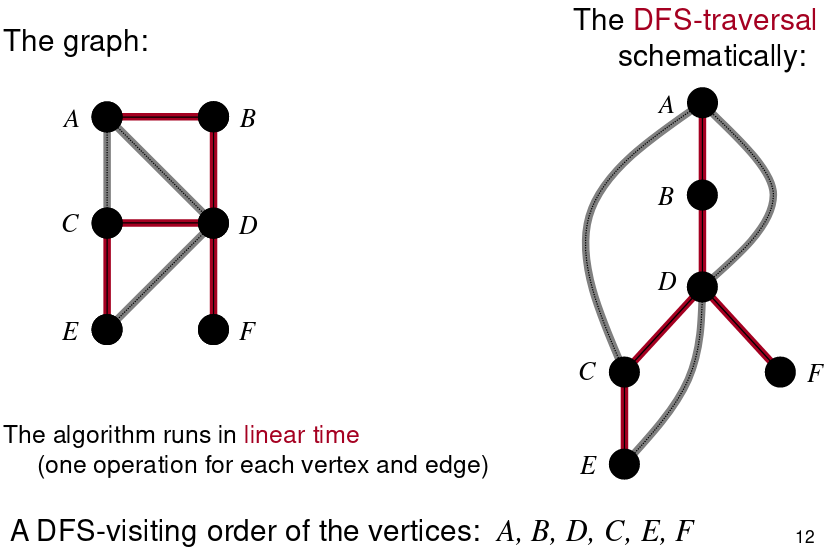
\includegraphics[scale=0.7]{DFS}
\end{center}
\section{Graph traversing}
\begin{itemize}
	\item The Depth First Search (DFS) algorithm can be used to traverse the whole graph
	\item It can also be used for directed graphs:
	\begin{itemize}
		\item In this case Adj[u] denotes the set of vertices that are accessible from u with one edge
	\end{itemize}
	\item Variations of DFS are mainly used for "connectivity type" problems
\end{itemize}
\section{Shortest Paths}
\begin{itemize}
	\item The length of a path connecting two vertices a,b is the number of edges in the path
	\item The distance between two vertices a,b in a graph is the smallest length of a path that connects a and b
	\item The shortest path problem: given two vertices a and b, what is their distance?
\end{itemize}
Sketch of a simple algorithm for shortest paths:
\begin{itemize}
	\item You stand on a vertex a of the graph and need to find your distance to the vertex b
	\item Ask all your neighbours what is their distance to b and compute the smallest of these distances, say x
	\item Then your distance to b is equal to $x+1$
\end{itemize}
\begin{center}
	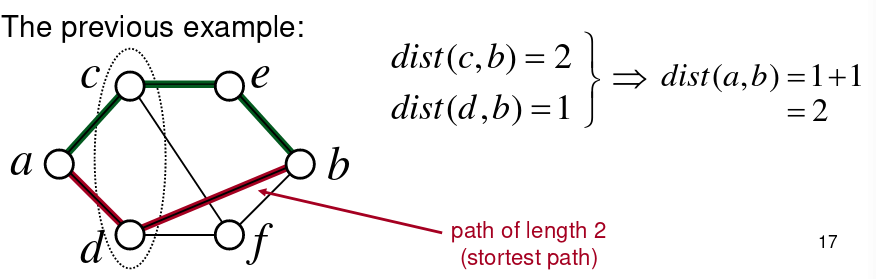
\includegraphics[scale=0.7]{Shortest}
\end{center}
In this algorithm, we proceed layer by layer:
\begin{itemize}
	\item We expand the "frontier" between visited and unvisited vertices, across the breadth of the frontier
	\begin{center}
		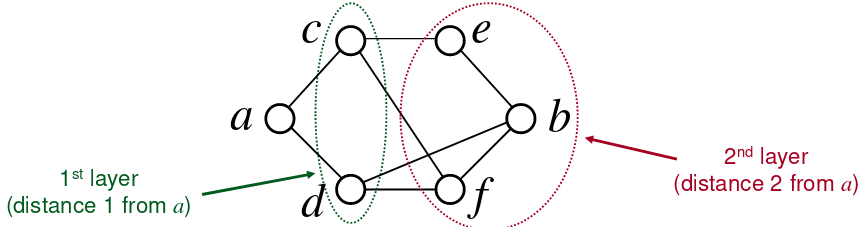
\includegraphics[scale=0.7]{Shortest1}
	\end{center}
	\item For every k=1,2,3 the algorithm:
	\begin{itemize}
		\item First visits all vertices at distance k from a
		\item Then all vertices at distance k+1
	\end{itemize}
\end{itemize}
\section{Breadth First Search (BFS)}
The natural alternative to DFS
\begin{lstlisting}
BFS(G,a,b)
i=0
label=[a]=0
while b is unlabeled
	for each vertex u with label[u]==i
		for each unlabeled vertex $v\in Adj[u]$
			label[v]=i+1
	i=i+1
return label[b]
\end{lstlisting}
\begin{itemize}
	\item BFS is an iterative algorithm, i.e. no recursive calls
	\item The label of a vertex u equals its distance from a
	\item We could continue iteration until all vertices are labelled
	\item Initially all vertices are marked a unlabelled i.e. label[u]= $-1$ or $\infty$
\end{itemize}
\section{BFS In action}
\begin{center}
	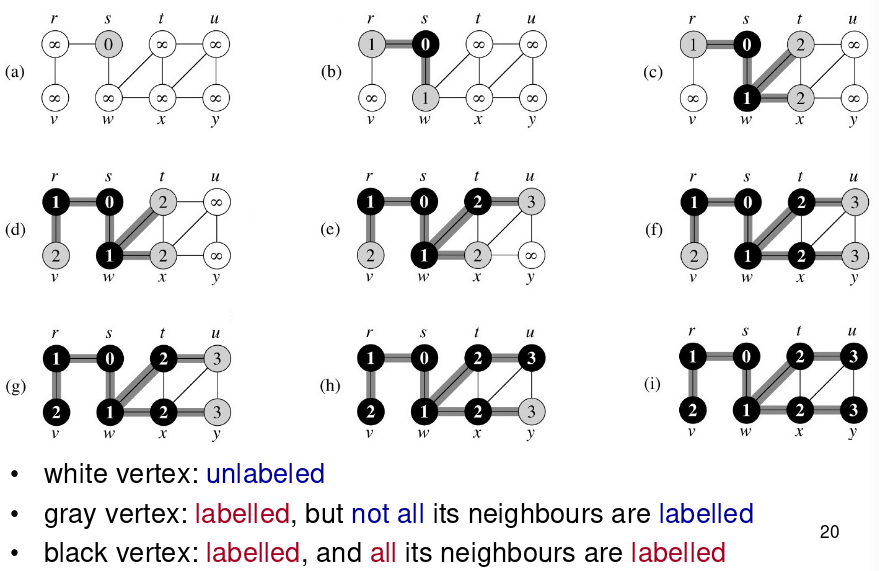
\includegraphics[scale=0.7]{BFS}
\end{center}

\end{document}